\documentclass[12pt]{amsart}
\usepackage{amsmath}
\usepackage{tikz,float,caption}
\usetikzlibrary{arrows.meta,calc,decorations.markings,patterns,cd,patterns.meta}

\begin{document}

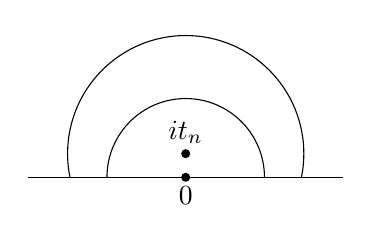
\begin{tikzpicture}
      \begin{scope}
        \clip (-2,0)rectangle (2,1.9);
        \draw (0,0.3) circle (3/2) node (A){};
        \draw (0,0) circle (1);
      \end{scope}
      \draw (-2,0)--(2,0);
      \node[draw,circle,fill,inner sep=1pt] (Z)at (0,0) {};
      \node[draw,circle,fill,inner sep=1pt] at (A) {};
      \node at (A) [above] {$it_{n}$};
      \node at (Z) [below] {$0$};
    \end{tikzpicture}

\end{document}